\chapter{Desarrollo Teórico y Simulación}
\label{sec.ej2:desarrollo}

\section{Modulación de Frecuencia (FM)}
En la modulación en frecuencia (FM), la frecuencia instantánea de la portadora se varía en forma lineal con la
amplitud de la señal modulante. La ecuación general que representa a una señal modulada en frecuencia, según la
expresión general del libro de Pedro E. Danizio (ecuación 4.2.8), es:
\begin{equation}
    e_{\text{FM}}(t) = E_c \cos\left(\omega_c t + K_f \int_0^t e_m(\tau) d\tau\right)
    \label{eq.ej2:fm_general}
\end{equation}
donde $E_c$ es la amplitud de la portadora, $\omega_c = 2\pi f_c$ es la frecuencia angular de la portadora, $K_f$ es
la sensibilidad del modulador en frecuencia (en $\text{rad}/(\text{s}\cdot\text{V})$), y $e_m(t)$ es la señal modulante.

En este trabajo práctico, se considera que tanto la señal modulante como la portadora son señales cosenoidales,
cuyas ecuaciones respectivas se plantean como:
\begin{equation}
    e_m(t) = E_m \cos(\omega_m t)
    \label{eq.ej2:em_cos}
\end{equation}
\begin{equation}
    e_c(t) = E_c \cos(\omega_c t)
    \label{eq.ej2:ec_cos}
\end{equation}
donde $E_m$ y $E_c$ representan las amplitudes pico, y $\omega_m = 2\pi f_m$ y $\omega_c = 2\pi f_c$ sus respectivas
frecuencias angulares.

Al integrar la señal modulante $e_m(t)$, tal como lo establece la ecuación general de la FM (ecuación
\ref{eq.ej2:fm_general}), se obtiene una función sinusoidal:
\begin{equation}
    \int_0^t e_m(\tau) d\tau = \int_0^t E_m \cos(\omega_m \tau) d\tau = \frac{E_m}{\omega_m} \sin(\omega_m t)
    \label{eq.ej2:em_integral}
\end{equation}

Sustituyendo esta integral en la ecuación general (\ref{eq.ej2:fm_general}), se obtiene la ecuación clásica
de la señal modulada en frecuencia para un tono sinusoidal:
\begin{equation}
    e_{\text{FM}}(t) = E_c \cos\left(\omega_c t + m_f \sin(\omega_m t)\right)
    \label{eq.ej2:fm_signal}
\end{equation}
donde $m_f$ es el índice de modulación en frecuencia, el cual se define en la teoría como:
\begin{equation}
    m_f = \frac{K_f E_m}{\omega_m} = \frac{\Delta\omega}{\omega_m} = \frac{\Delta f}{f_m}
    \label{eq.ej2:beta}
\end{equation}
siendo $\Delta\omega = K_f E_m$ la desviación máxima de frecuencia angular y $\Delta f = \Delta\omega / 2\pi$ la
desviación máxima en frecuencia (en $\Hz$).

Para las condiciones de simulación, se establecen los siguientes parámetros de diseño:
\begin{itemize}
    \item Frecuencia de portadora: $f_c = 10\kHz$ ($\omega_c = 2\pi \cdot 10\text{ krad/s}$)
    \item Frecuencia modulante: $f_m = 1\kHz$ ($\omega_m = 2\pi \cdot 1\text{ krad/s}$)
    \item Índice de modulación: $m_f = 5$
    \item Amplitud de portadora: $E_c = 1\V$
    \item Amplitud de modulante: $E_m = 1\V$
\end{itemize}

A partir de estos valores, la desviación máxima de frecuencia es:
\begin{equation*}
    \Delta f = m_f \cdot f_m = 5 \cdot 1\kHz = 5\kHz
\end{equation*}
La frecuencia instantánea de la señal variará de forma sinusoidal entre un valor mínimo y uno máximo:
\begin{align*}
    f_{\text{mín}} &= f_c - \Delta f = 10\kHz - 5\kHz = 5\kHz \\
    f_{\text{máx}} &= f_c + \Delta f = 10\kHz + 5\kHz = 15\kHz
\end{align*}

El ancho de banda de transmisión de la señal FM se puede estimar mediante la regla de Carson:
\begin{equation}
    B_C = 2(\Delta f + f_m) = 2(m_f + 1)f_m
    \label{eq.ej2:carson}
\end{equation}
Sustituyendo los valores de simulación:
\begin{equation*}
    B_C = 2(5\kHz + 1\kHz) = 12\kHz
\end{equation*}
El espectro de potencia significativo se distribuye en el rango de frecuencias de $4\kHz$ a $16\kHz$.

\section{Demodulación por Derivación}
El demodulador propuesto emplea un bloque derivador para transformar la modulación de frecuencia en modulación de
amplitud. La derivada temporal de la señal FM (ecuación \ref{eq.ej2:fm_signal}) está dada por:
\begin{equation*}
    e_B(t) = \frac{d e_{\text{FM}}(t)}{dt} = - E_c \left[\omega_c + K_f E_m \cos(\omega_m t)\right]
    \sin\left(\omega_c t + m_f \sin(\omega_m t)\right)
\end{equation*}
Extrayendo como factor común el término constante de frecuencia de portadora $\omega_c$:
\begin{equation}
    e_B(t) = - E_c \omega_c \left[1 + \frac{K_f E_m}{\omega_c} \cos(\omega_m t)\right]
    \sin\left(\omega_c t + m_f \sin(\omega_m t)\right)
    \label{eq.ej2:derivada}
\end{equation}
La ecuación \ref{eq.ej2:derivada} representa una señal que posee modulación tanto en amplitud como en frecuencia.
La envolvente de esta señal es:
\begin{equation}
    E(t) = E_c \omega_c \left| 1 + \frac{K_f E_m}{\omega_c} \cos(\omega_m t) \right|
    \label{eq.ej2:envolvente}
\end{equation}
Esta expresión muestra que la envolvente de la señal derivada es directamente proporcional a la señal modulante
sinusoidal $e_m(t) = E_m \cos(\omega_m t)$. Por lo tanto, un detector de envolvente asincrónico convencional puede
recuperar la información original a partir de $E(t)$.

\section{Condición de No Distorsión}
Esta condición surge de la necesidad de evitar la distorsión al derivar una señal modulada para demodularla, proceso que resulta en una señal con modulación de amplitud. Por lo tanto, para evitar la distorsión al derivar (al demodular), se debe evitar la distorsión de la señal AM. En la modulación AM, si el índice de modulación es mayor que 1, la amplitud de la modulante supera a la portadora y se produce distorsión, arruinando la recepción mediante un detector de envuelta. Para garantizar que no haya distorsión en nuestra señal derivada, su índice equivalente debe ser menor o igual a uno.

En la expresión de la envolvente que resulta al derivar (ecuación \ref{eq.ej2:envolvente}), el término $\frac{K_f E_m}{\omega_c}$ equivale a $\frac{\Delta\omega}{\omega_c}$ (donde $\Delta\omega = K_f E_m$ es la desviación de frecuencia angular). Este término actúa como el índice de modulación de la envolvente, el cual podemos denotar como $\delta = \frac{\Delta\omega}{\omega_c}$. Aplicando directamente la condición $\delta \le 1$ (o equivalentemente, $\frac{\Delta\omega}{\omega_c} \le 1$) para evitar la distorsión, se garantiza que la envolvente nunca tome valores negativos ni cruce por cero. Dado que $\Delta\omega = m_f \cdot \omega_m$, esta condición equivale a exigir que:
\begin{equation*}
    m_f \le \frac{\omega_c}{\omega_m} = \frac{f_c}{f_m}
\end{equation*}

Para las frecuencias del circuito en estudio ($f_c = 10\kHz$ y $f_m = 1\kHz$), el máximo índice de modulación permitido sin que se produzca distorsión en la señal demodulada es:
\begin{equation*}
    m_{f,\text{máx}} = \frac{10\kHz}{1\kHz} = 10
\end{equation*}

Si el índice de modulación supera este límite ($m_f > 10$), la amplitud de la portadora derivada se vuelve negativa en
ciertos intervalos de tiempo. Esto representa una sobremodulación de la componente AM, generando una inversión de
fase en la señal de portadora. Dado que el rectificador de media onda responde únicamente al valor absoluto de la
envolvente, la señal rectificada presentará distorsión armónica severa (deformación en los cruces por cero), la cual
no podrá ser eliminada por el filtro paso bajo posterior, distorsionando la señal de salida.

\section{Análisis de los Resultados de Simulación}
El circuito de simulación propuesto se muestra en la figura \ref{fig.ej2:schematic}. Consta de un generador de FM,
un derivador analógico ($A_1$), un buffer de tensión ($A_2$), un diodo detector virtual ($D_1$), una resistencia
de carga ($R_1 = 10\kohm$) y un filtro paso bajo activo ($HB_1$) con frecuencia de corte de $1\kHz$.

\begin{figure}[!ht]
    \centering
    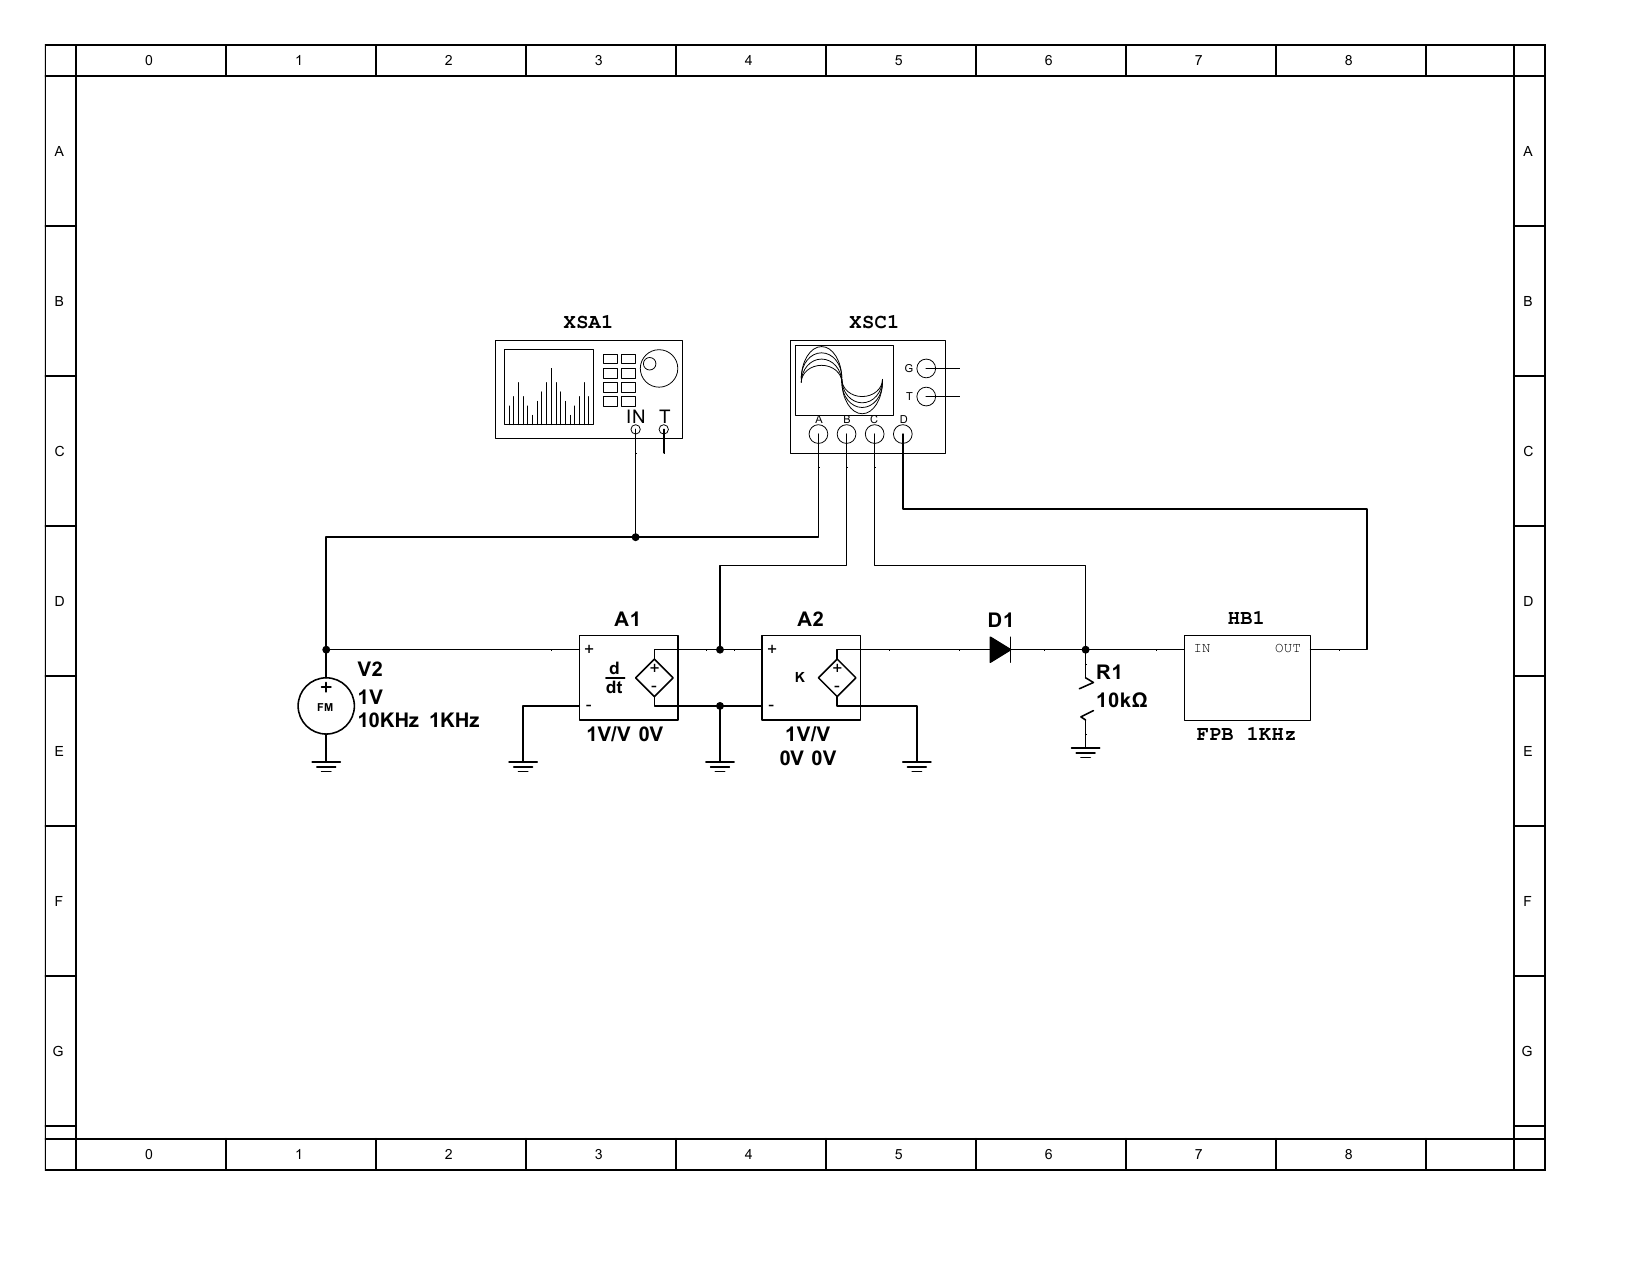
\includegraphics[width=0.9\textwidth]{images/multisim_circuit-1.png}
    \caption{Esquema del modulador y demodulador de FM implementado en Multisim.}
    \label{fig.ej2:schematic}
\end{figure}

El análisis temporal de las señales en los diferentes puntos de medición se realizó utilizando el osciloscopio
de cuatro canales, obteniendo las formas de onda presentadas en la figura \ref{fig.ej2:oscilloscope}.

\begin{figure}[!ht]
    \centering
    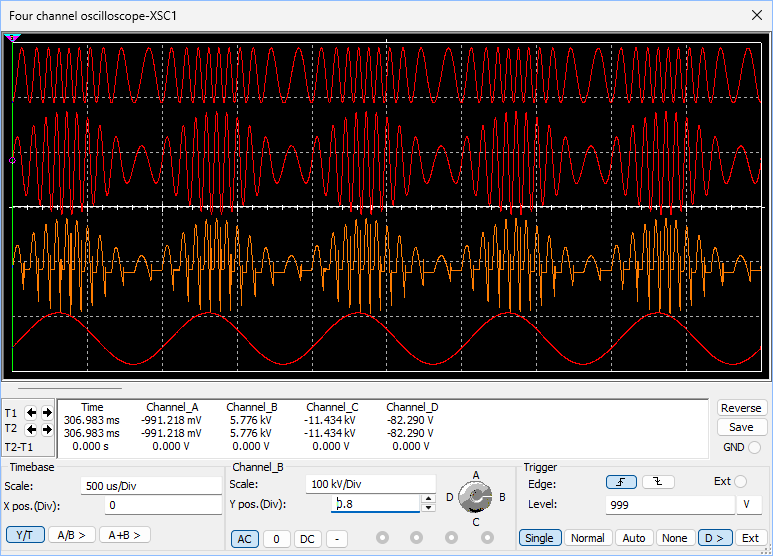
\includegraphics[width=0.9\textwidth]{images/oscilloscope.png}
    \caption{Formas de onda en los puntos de medición del osciloscopio XSC1.}
    \label{fig.ej2:oscilloscope}
\end{figure}

Las señales observadas corresponden a:
\begin{description}
    \item[Canal A (rojo - superior)] Señal FM modulada en el punto de medición A. Se observa que la amplitud se
          mantiene constante en $1\V$, mientras que la frecuencia varía de forma continua entre el valor mínimo
          de $5\kHz$ (zonas de menor densidad de oscilaciones) y el máximo de $15\kHz$ (zonas de mayor densidad).
    \item[Canal B (rojo - intermedio)] Señal a la salida del derivador (punto B). Se verifica el efecto de la
          derivación: la amplitud de la señal ahora varía en función de la frecuencia instantánea. Los picos de
          amplitud coinciden con las frecuencias más altas de la señal FM original (mayor pendiente en la derivada),
          mientras que los valles coinciden con las frecuencias más bajas. Esto confirma el carácter AM-FM de la señal.
    \item[Canal C (naranja)] Señal rectificada a la salida del diodo detector (punto C). La señal presenta una
          rectificación de media onda, eliminando los semiciclos negativos de la portadora derivada. Esto permite
          aislar la envolvente de la señal de alta frecuencia para su posterior filtrado.
    \item[Canal D (rojo - inferior)] Señal de salida del filtro paso bajo (punto D). El filtro elimina las
          componentes espectrales de la portadora y sus armónicos de rectificación, entregando una señal sinusoidal
          limpia de $1\kHz$, que coincide perfectamente en frecuencia y fase con la señal modulante original.
\end{description}

\section{Análisis en Frecuencia}
El espectro de la señal FM modulada se midió con el analizador de espectro, como se ilustra en la figura
\ref{fig.ej2:spectrum}.

\begin{figure}[!ht]
    \centering
    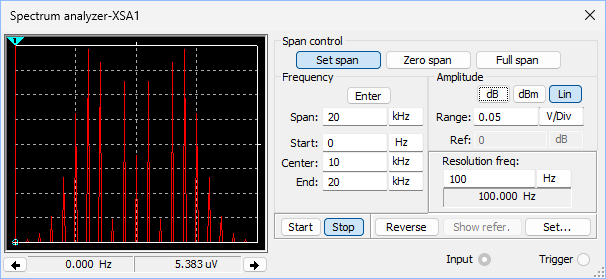
\includegraphics[width=0.8\textwidth]{images/spectrum.png}
    \caption{Espectro de la señal FM modulada medido en el punto de medición A.}
    \label{fig.ej2:spectrum}
\end{figure}

En el espectro se observa la componente central correspondiente a la portadora en $10\kHz$ y componentes laterales
simétricas espaciadas a intervalos de $1\kHz$ (frecuencia de la modulante $f_m$). La distribución de amplitudes
sigue el comportamiento teórico de las funciones de Bessel de primera especie de orden $n$, $J_n(m_f)$, para
un índice de modulación $m_f = 5$. 

Se puede comprobar que el ancho de banda efectivo cumple de forma rigurosa con la regla de Carson. Las líneas
espectrales significativas con amplitudes no despreciables se extienden aproximadamente desde $4\kHz$ hasta $16\kHz$,
lo cual concuerda con el ancho de banda calculado de $12\kHz$ y valida experimentalmente el comportamiento espectral
teórico de la señal modulada en frecuencia.
